\documentclass[final,hyperref={pdfpagelabels=false}]{beamer}
\usepackage{grffile}
\mode<presentation> {\usetheme{I6pd2}}
\usepackage[english]{babel}
\usepackage[latin1]{inputenc}
\usepackage{amsmath,amsthm, amssymb, latexsym}
%\usepackage{times}\usefonttheme{professionalfonts}  % obsolete
\usefonttheme[onlymath]{serif}
\boldmath
\usepackage[orientation=landscape,size=a0,scale=1.4,debug]{beamerposter}
% change list indention level
% \setdefaultleftmargin{3em}{}{}{}{}{}


%\usepackage{snapshot} % will write a .dep file with all dependencies, allows for easy bundling

\usepackage{array,booktabs,tabularx}
\newcolumntype{Z}{>{\centering\arraybackslash}X} % centered tabularx columns
%\newcommand{\pphantom}{\textcolor{ta3aluminium}} % phantom introduces a vertical space in p formatted table columns??!!

\listfiles

%%%%%%%%%%%%%%%%%%%%%%%%%%%%%%%%%%%%%%%%%%%%%%%%%%%%%%%%%%%%%%%%%%%%%%%%%%%%%%%%%%%%%%
\graphicspath{{figures/}}
 
\title{\huge Performance of PyCUDA \\ \LARGE(Python in GPU High Performance Computing)}
\author{\textcolor{azulpastel}{Roberto Colistete Jr and Ramon Giostri Campos}}
\institute[UFES]{UFES, Brazil}
\date[Data]{Data novamente}

%%%%%%%%%%%%%%%%%%%%%%%%%%%%%%%%%%%%%%%%%%%%%%%%%%%%%%%%%%%%%%%%%%%%%%%%%%%%%%%%%%%%%%
\newlength{\columnheight}
\setlength{\columnheight}{105cm}


%%%%%%%%%%%%%%%%%%%%%%%%%%%%%%%%%%%%%%%%%%%%%%%%%%%%%%%%%%%%%%%%%%%%%%%%%%%%%%%%%%%%%%

%\setbeamertemplate{blocks}[rounded] [shadow=false]

\begin{document}
\begin{frame}
 \vspace{.005\columnheight}
  \begin{columns}
    % ---------------------------------------------------------%
    % Set up a column 
    \begin{column}{.245\textwidth}
      \begin{beamercolorbox}[center,wd=\textwidth]{postercolumn}
        \begin{minipage}[T]{.95\textwidth}  % tweaks the width, makes a new \textwidth
          \parbox[t][\columnheight]{\textwidth}{ % must be some better way to set the the height, width and textwidth simultaneously
            % Since all columns are the same length, it is all nice and tidy.  You have to get the height empirically
            % ---------------------------------------------------------%
            % fill each column with content            
            \begin{block}{Introduction}
              High Performance Computing with GPU (Graphics Processing Unit) and CUDA (Compute Unified Device Architecture) can be made using Python via PyCUDA. Here we will compare PyCUDA versus C, CUDA, Python and Wolfram Mathematica in a calculation example from type Ia supernova cosmology.
              
              Advances in computational techniques have allowed to explore issues related to science and technology that were previously unimaginable, one of them is the development of parallel computing using GPU.
              
              We target the problem of calculating the distance modulus $(\mu_0)$ for type Ia supernovae (SNe Ia) for the case of flat standard model of cosmology[1], when it has $N=3$ free parameters. Under these conditions  the calculation is performed about $10^3$ times for each supernova. But for supported models with $N$ dimensions, it can vary between $10^N$ to $10^{2N}$. Also worth remembering is that today the supernovae catalogs are of the order of a thousand supernovae and the estimate is that with new experiments it will have hundreds of thousands of SNe Ia in a few years[2]. Given the values shown we have a very intensive computational problem.
                            
              In this context, we perform the calculation of the distance modulus $(\mu_0)$ using C, C/CUDA, Python/ Numpy, PyCUDA and Wolfram Mathematica (without and with CUDA), clearly showing the advantages and disadvantages of these approaches.
                          
            \end{block}
            \vspace{.005\columnheight}
  			\begin{block}{Physical Problem}
              A supernova is one of the possible final stages of a star, there are several types of supernovae[3] and we give particular attention to the type Ia supernovae (SNe Ia). The SNe Ia are standardizable candles and this feature was essential to prove that the universe expands with acceleration in 1998/1999[4,5], this pioneering work have won the Nobel prize in 2011.
              Calculation of the theoretical distance modulus $\mu_0$ is a central part of SNe Ia observational cosmology, as it is the amount statistically compared with the astronomical observable:
%      \vspace{.003\columnheight}
            {\small  \[
             \mu_0(z,\Theta)=25+5\,log_{10}\left( \frac{(1+z)c}{H_0}\int_{0}^{z}\frac{1}{h(z',\Theta)}dz' \right) 
             \]}
%       \vspace{.003\columnheight}
             For flat cosmological models the changes are in the denominator of integrand, for non flat models, more significant changes are necessary[6].
             \end{block}
          }
        \end{minipage}
      \end{beamercolorbox}
    \end{column}
    % ---------------------------------------------------------%
    % end the column

    % ---------------------------------------------------------%
    % Set up a column 
    \begin{column}{.49\textwidth}
      \begin{beamercolorbox}[center,wd=\textwidth]{postercolumn}
        \begin{minipage}[T]{.95\textwidth} % tweaks the width, makes a new \textwidth
          \parbox[t][\columnheight]{\textwidth}{ % must be some better way to set the the height, width and textwidth simultaneously
            % Since all columns are the same length, it is all nice and tidy.  You have to get the height empirically
            % ---------------------------------------------------------%
            % fill each column with content
            
                \begin{columns}
                  \begin{column}{.45\textwidth}
                    \begin{block}{Benefits of PyCUDA}
             	      \begin{itemize}
                       	\item DP (Double Precision) as fast as C/CUDA
                       	\item Hundreds times faster than NumPy
                       	\item Faster than Wolfram Mathematica with CUDA, no issues with SP (Single Precision)
                       	\item Easier to write, less code than pure C/CUDA
                       	\item Allows metaprogramming
                       	\item Free and open source, while Wolfram Mathematica is not
                      \end{itemize}
                    \end{block}
                  \end{column}
                  \begin{column}{.45\textwidth}
                    \begin{block}{Drawbacks of PyCUDA}
                      \begin{itemize}
                        \item SP (Single Precision) slower than C/CUDA
                        \item Kernel is still written in C/CUDA
                        \item Additional installation, sometimes with dependency issues
                      \end{itemize}
                    \end{block}
                  \end{column}
                \end{columns}
            
                \vspace{.005\columnheight}
            
            \begin{block}{Performance of $\mu_0$ Calculations in GPU and CPU}
              {\small Made on a workstation with Intel Core i7 4770K (3.5-3.9 GHz, 8MB cache, 4 cores, 8 threads), 16GB RAM, GeForce GTX Titan (2,688 cores, 6GB GDDR5 RAM), Ubuntu 14.04.2 64 bits, Linux kernel 3.16.0, gcc 4.8.4, Python 2.7.6, NumPy 1.8.2, CUDA 7.0-28, PyCUDA v2015.1, Mathematica 10.1 :}
              \vspace{0.2cm}
              \begin{columns}
                \begin{column}{.45\textwidth}
                  \begin{exampleblock}{\small \centering Comparison of \textcolor{blue}{CUDA}, \textcolor{orange}{PyCUDA}  in SP $\times$ C}
                    \begin{center}
                      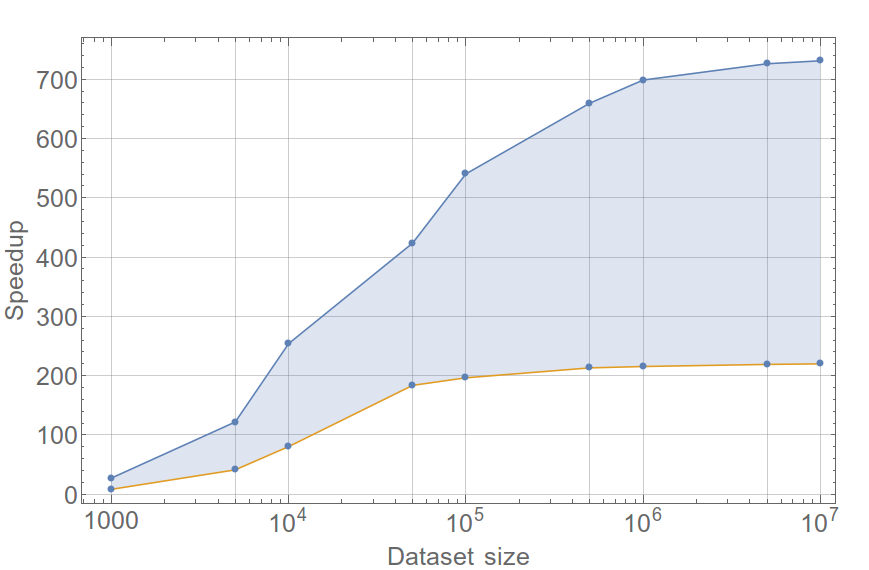
\includegraphics[scale=0.8]{Grafico_ganho_x_num_SP.png}
                    \end{center}
                  \end{exampleblock}
                \end{column}
                \begin{column}{.45\textwidth}
                  \begin{exampleblock}{\small \centering Comparison of \textcolor{blue}{CUDA}, \textcolor{orange}{PyCUDA}, \textcolor{green}{WMC} in DP $\times$ C}
                    \begin{center}
                      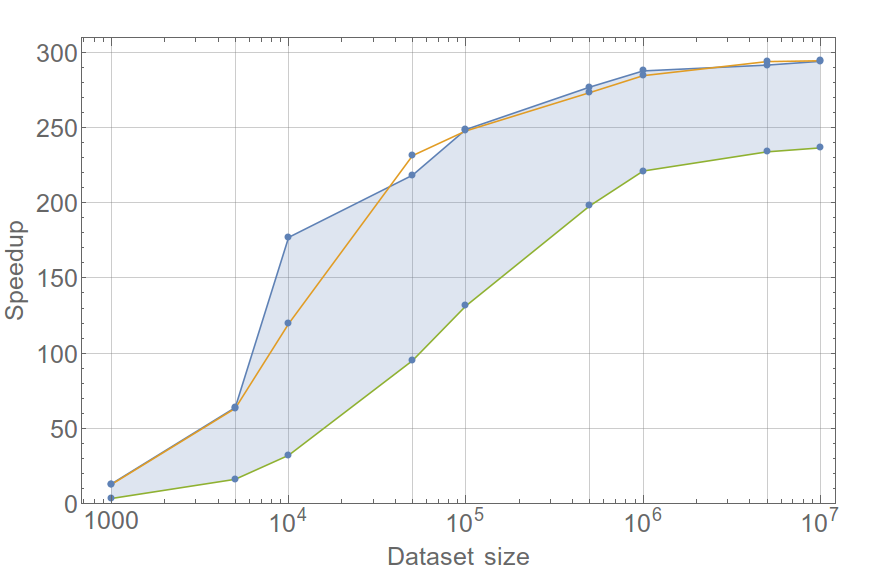
\includegraphics[scale=0.8]{Grafico_ganho_x_num_DP.png}
                    \end{center}
                  \end{exampleblock}
                \end{column}                                
              \end{columns}
              \vspace{0.2cm}
              {\small Speedup with respect C/C++ (in 1 CPU core) vs. dataset size (number of supernovae) in SP (Single Precision) and DP (Double Precision). WMC : Wolfram Mathematica 10.1 using CUDA, which doesn't work in SP.}
              \vspace{.005\columnheight}
              \begin{columns}
              \begin{column}{.95\textwidth}
                \begin{exampleblock}{$\mu_0$ calculation time in DP for $10^5$ SNe Ia}
                  \begin{table}
               	    %\begin{tabular}{|c|c|c|c|c|c|c|}
                    \begin{tabular}{@{} p{.17\linewidth} | p{.10\linewidth} p{.12\linewidth} p{.10\linewidth} p{.10\linewidth} p{.10\linewidth} p{.10\linewidth} p{.08\linewidth} r r r r r r r r @{}}
                      \textbf{Method} &\textbf{CUDA} &\textbf{PyCUDA} &\textbf{WMC} &\textbf{C/C++} &\textbf{Python}  &\textbf{NumPy} & \textbf{WM} \\ 
                      \toprule \textbf{Total time (s)} & 0.002941 & 0.002952 & 0.006366 & 0.7327 & 46.13 & 1.499 & 2.634  \\ 
                   	  \toprule \textbf{Kernel time (s)} & 0.002576 & 0.002450 & 0.003632 & --- & --- & --- & --- \\ 
                    \end{tabular} 
                  \end{table}
                \end{exampleblock}
                {\small $\mu_0$ calculation time in DP (Double Precision) for $10^5$ SNe Ia. WMC : Wolfram Mathematica 10.1 using CUDA. WM : Wolfram Mathematica 10.1 using CPU. Python : pure Python. NumPy : Python with NumPy. }
              \end{column}                                
            \end{columns}
          \end{block}
            \vspace{.005\columnheight}
            %\vfill
            \begin{block}{Performance Analysis}
%              \vskip1ex
               In SP (Single Precision), C/CUDA is 1-2 times faster than PyCUDA because PyCUDA has overhead in dealing with SP data. While Wolfram Mathematica versions 9/10 don't calculate at all when running kernels in SP.
               
               In DP (Double Precision), PyCUDA is approximately as fast as C/CUDA. Both are faster than Wolfram Mathematica with CUDA, which is not efficient in CPU-GPU communication.
            \end{block}
           % \vfill
          }
          % ---------------------------------------------------------%
          % end the column
        \end{minipage}
      \end{beamercolorbox}
    \end{column}
    \begin{column}{.245\textwidth}
      \begin{beamercolorbox}[center,wd=\textwidth]{postercolumn}
        \begin{minipage}[T]{.95\textwidth} % tweaks the width, makes a new \textwidth
          \parbox[t][\columnheight]{\textwidth}{ % must be some better way to set the the height, width and textwidth simultaneously
            % Since all columns are the same length, it is all nice and tidy.  You have to get the height empirically
            %     
             \begin{block}{Conclusion}
               PyCUDA let us use CUDA (Compute Unified Device Architecture) from Python, making High Performance Computing (HPC) with GPU (Graphics Processing Unit) easier with respect to C/C++ with CUDA, while being robust and giving good performance.
               
               Wolfram Mathematica, which has an interpreted language, can also call CUDA since version 8, so it (in version 10) was compared here.
			   
			   Performance wise in SP (Single Precision), C/CUDA speedup w.r.t. C/C++ (CPU using 1 core) is up to 730 times. PyCUDA speedup w.r.t. C/C++ is up 220 times, w.r.t. Python/NumPy is up to 450 times. So C/CUDA is 1-2 times faster than PyCUDA in SP.
               
               In DP (Double Precision), PyCUDA is approximately as fast as C/CUDA : C/CUDA speedup w.r.t. C/C++ is up to 294 times. PyCUDA speedup w.r.t. C/C++ is up 294 times, w.r.t. Python/NumPy is up to 601 times. Wolfram Mathematica with CUDA speedup w.r.t. C/C++ is up to 237, w.r.t. to Mathematica (using CPU) is up to 852 times.
               
               So PyCUDA compares very well, being : as fast as C/CUDA in Double Precision (DP); faster and more robust than Wolfram Mathematica with CUDA; hundreds times faster than C/C++, pure Python, Python with NumPy, and Wolfram Mathematica calculated in CPU.
               
               We conclude that PyCUDA has many advantages, so it is the logical step for Python developers coming from CPU calculations with Python/NumPy and going to use GPU programming.
             \end{block}
             \vspace{.005\columnheight}

			 \begin{block}{Acknowledgments}
				{\small R. Colistete Jr. thanks the SciPy 2015 Conference organization for the hospitability and financial support.}
			 \end{block}
             \vspace{.005\columnheight}

			\begin{block}{References}
		{\footnotesize 	\begin{description}
			\item[1] Wang et al., Dark Energy, Wiley, Weinheim, Germany, 2010.
			\item[2] Weinberg et al., Observational Probes of Cosmic Acceleration, 2012.
			\item[3] Filippenko, OPTICAL SPECTRA OF SUPERNOVAE, 1997.
			\item[4] Riess et al., Observational Evidence from Supernovae for an Accelerating Universe and a Cosmological Constant, 1998.
			\item[5] Permutter et al., Measurements of $\Omega$ and $\Lambda$ from 42 HighRedshift Supernovae, 1999.
			\item[6] Persis et al. Type Ia supernovae, evolution, and the cosmological constant, 1999.
			\end{description}}
			\end{block}
          }
          % ---------------------------------------------------------%
          % end the column
        \end{minipage}
      \end{beamercolorbox}
    \end{column}            
         
    % ---------------------------------------------------------%
    % end the column
  \end{columns}
  \vskip1ex
  %\tiny\hfill\textcolor{ta2gray}{Created with \LaTeX \texttt{beamerposter}  \url{http://www-i6.informatik.rwth-aachen.de/~dreuw/latexbeamerposter.php}}
  \tiny\hfill{Created with \LaTeX \texttt{beamerposter}  \url{Sua url} \hskip1em}
\end{frame}
\end{document}


%%%%%%%%%%%%%%%%%%%%%%%%%%%%%%%%%%%%%%%%%%%%%%%%%%%%%%%%%%%%%%%%%%%%%%%%%%%%%%%%%%%%%%%%%%%%%%%%%%%%
%%% Local Variables: 
%%% mode: latex
%%% TeX-PDF-mode: t
%%% End:
